\documentclass[10pt,a4paper]{article}

\usepackage{polski}
\usepackage[utf8]{inputenc}
\usepackage[polish]{babel}
\usepackage{hhline}
\usepackage{pgfplots}
\usepackage{multicol}
\usepackage{graphicx}
\usepackage{caption}
\usepackage{subcaption}
\usepackage{colortbl}
\usepackage{geometry}
\usepackage{listings}
\usepackage{mathtools}
\DeclarePairedDelimiter\ceil{\lceil}{\rceil}
\DeclarePairedDelimiter\floor{\lfloor}{\rfloor}
\geometry{a4paper, total={170mm,257mm}, left=20mm, top=20mm }


\author{Sebastian Maciejewski 132275 i Jan Techner 132332\\
grupa I1, zajęcia w środy o 9:45}
\title{Przetwarzanie rozproszone - projekt “Obsługa Pyrkonu”}
\date{15 maja 2019}
\setlength{\parindent}{0pt}
\newcommand{\forceindent}{\leavevmode{\parindent=3em\indent}}
\begin{document}
\maketitle
\section{Opis problemu}
Zadanie polega na implementacji systemu zarządzania biletami na Pyrkon i warsztaty, które się na nim odbywają. Procesy (uczestnicy) ubiegają się o jeden z b biletów na Pyrkon,
a następnie na kilka z rozróżnialnych warsztatów, z których każdy ma ograniczoną liczbę miejsc. Liczba warsztatów, miejsc na warsztatach i biletów na Pyrkon jest
w naszej implementacji losowana przez proces, który uruchamia wątek rozpoczęcia Pyrkonu.
Poniżej przedstawiony jest schemat działania i opis algorytmu.
\newpage
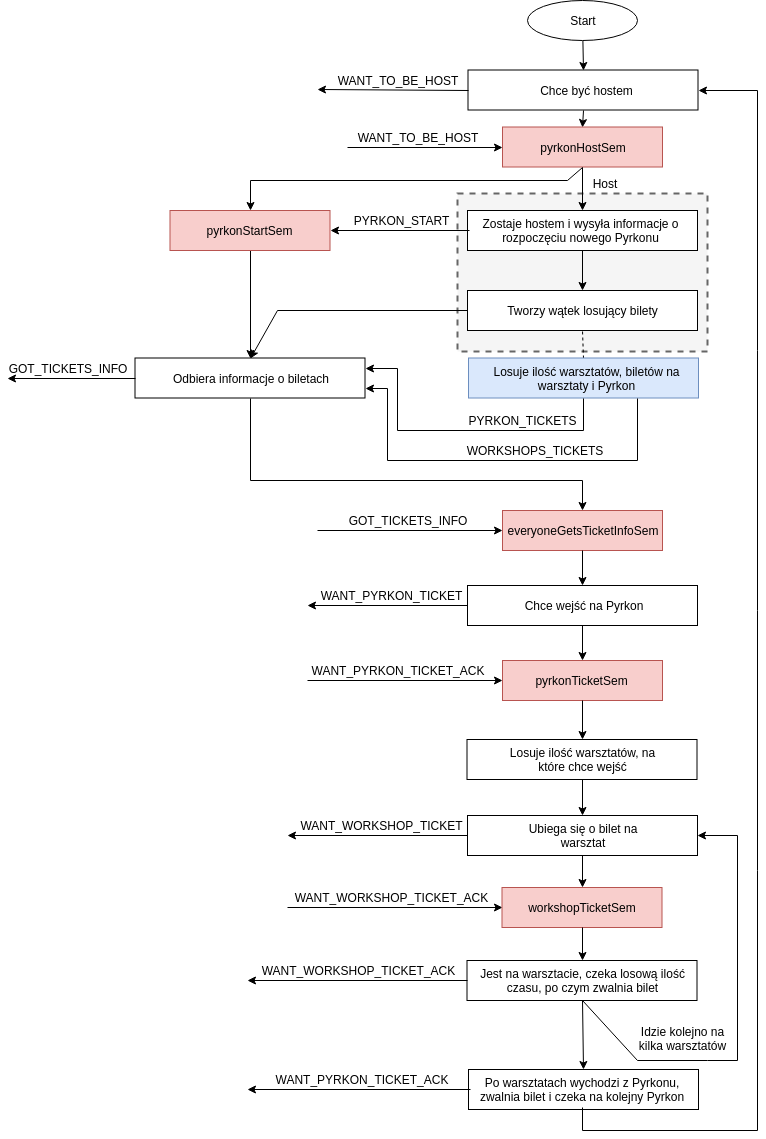
\includegraphics[height=\textheight]{diagram.png}


\end{document}